\subsection{CU3 Visualizar Agenda}
Supongamos que el usuario decide ver todos los registros de los vehículos dentro del taller y elige la opción de Gestionar Agenda, inmediatamente esta pantalla (figura \ref{fig:Pantalla Visualizar Agenda - Vista de Escenarios}) aparecerá. Compuesta principalmente por una tabla donde se mostrarán a manera de lista cada uno de los registros que estén almacenados en la base de datos, en caso de que no exista ningún registro, dicha tabla se mostrará vacía.
\\
En la parte superior derecha hay una barra de búsqueda, se explica a detalle este proceso mas adelante (véase \ref{sub:buscar registro}). 
\\
En la parte inferior se despliegan una serie de botones que permitirán al usuario gestionar esta tabla de registros que se le presentan:
\begin{itemize}
	\item \textbf{Actualizar Registro:} Permite al usuario actualizar la tabla una vez que este haya realizado algún cambio en los registros.
	\item \textbf{Registrar Vehículo:} Despliega una pantalla con un formulario de registro.
	\item \textbf{Modificar Vehículo:} Despliega una pantalla con un formulario de actualización.
	\item \textbf{Eliminar Vehículo:} Despliega una pantalla con un 'mensaje de seguridad'. 
	\item \textbf{Salir:} Regresar al menú de opciones (figura \ref{fig:Pantalla Visualizar Menu - Vista de Escenarios}). 
\end{itemize}
\begin{figure}[!h]
	\centering
	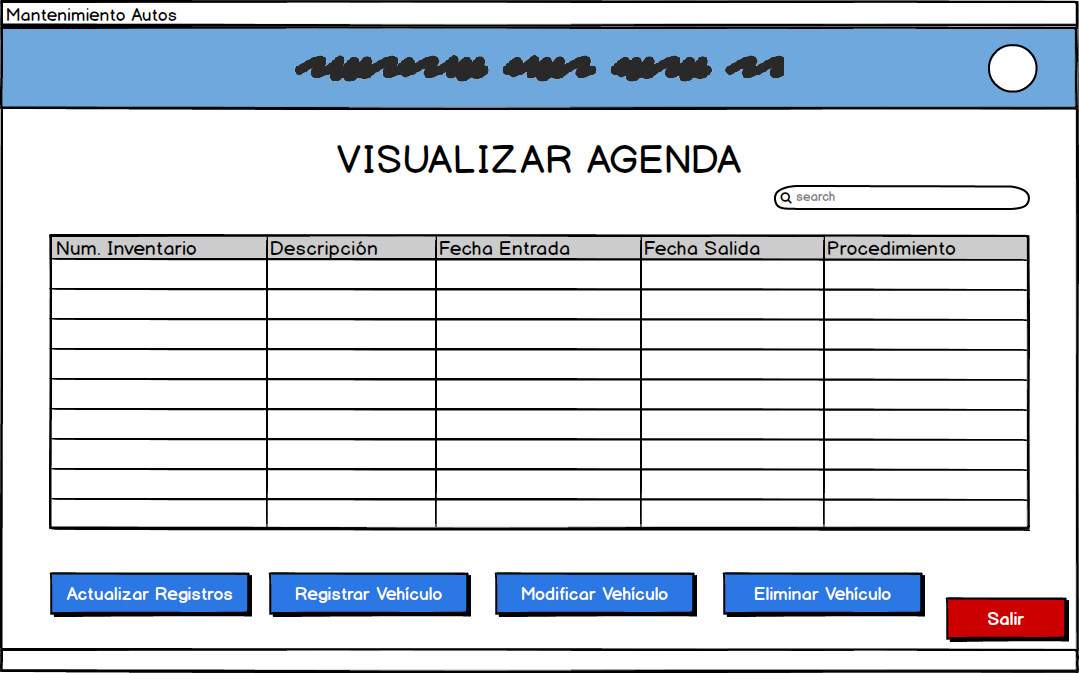
\includegraphics[width=1\textwidth]{./diseno/vescenarios/imagenes/VisualizarAgenda}
	\caption{Pantalla Visualizar Agenda - Vista de Escenarios}
	\label{fig:Pantalla Visualizar Agenda - Vista de Escenarios}
\end{figure}
Cabe señalar que el usuario debe de elegir un registro en la tabla para poder realizar alguna de las acciones antes mencionadas, de lo contrario aparecerá un 'mensaje de alerta' (figura \ref{fig:Alerta - Vista de Escenarios}) donde le de a entender al usuario lo que debe de hacer antes de relizar cualquier acción sobre algún registro.
\begin{figure}[!h]
	\centering
	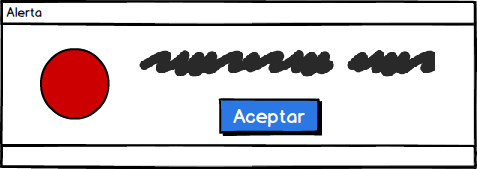
\includegraphics[width=0.5\textwidth]{./diseno/vescenarios/imagenes/alerta}
	\caption{Alerta Elección de Registro - Vista de Escenarios}
	\label{fig:Alerta - Vista de Escenarios}
\end{figure}
\clearpage